\chapter{Data Processing}
\label{ch:data_processing}
\graphicspath{{data_processing/}}
Super-Kamiokande records around $10^6$ events per day.  However, the vast majority of these events are either low energy radioactive backgrounds (~11 Hz) or cosmic ray muons (~3 Hz).  For comparison, the rate of atmospheric neutrino interactions in SK is about 10 per day.  Data reduction processes are used to select only the reatively small number of interesting physics events.  In the high energy range ($>100 MeV$), three samples are used, each selected by a separate data reduction process:
\begin{itemize}
\item Fully Contained (FC):  These are events with activity in the ID and no activity in the OD.  These events are the best reconstructed, since all the energy of the event is contained within the ID.
\item Partically Contained (PC):  These are events with activity in both the ID and OD, but where it has been determined that this is due to a particle starting in the ID and exiting into the OD.  These events are almost all muons, since most electromagnetic showers will not have the energy to puncture from the FV into the OD.  These events are more poorly reconstructed than FC events, since much of their energy can be deposited outside the ID, and even outside the OD.
\item Upward Going Muons (UPMU):  These are events with activity in both the ID and the OD, where the event starts in the OD, but where the event is coming from below the detector.  Since these events come from below, the Earth itself is acting as a shield for the detector.  The events are thus due to neutrinos interacting in the rock below the detector.
\end{itemize}

In this chapter, I will discuss all three of these reduction samples.
\section{Fully Contained Reduction}
\label{sec:FC}
The FC data reduction consists of five steps, labeled FC1-FC5.  Combined, they select around 8 events per day from the $10^6$ events recorded by SK, with an efficiency for selecting events which originate in the FV of about 98\%.  In the following descriptions, events which pass the cuts listed are the events which make up the FC sample.
\subsection{FC1}
FC1 consists of a two simple cuts:
\begin{itemize}
\item The number of pe in a 300 ns sliding time window in the ID is greater than 200 (100 for SK-II)
\item There are fewer than 50 (55 for SK-IV) OD hits between -500 ns and +300 ns.
\end{itemize}
The first cut removes low energy radioactive background events and solar neutrinos, while the second cut removes obvious cosmic ray muon and PC or UPMU events.  Of the $10^6$ events recorded by SK each day, about 3,500 pass FC1.

\subsection{FC2}
FC2 also consists of two simple cuts:
\begin{itemize}
\item No ID PMT can be responsible for greater than 50\% of the pe observed in the ID
\item If the number of pe in the ID is less than 100,000 (50,000 for SK-II), there must be fewer than 25 hits in the OD between -500 ns and +300 ns (30 for SK-IV).
\end{itemize}
This first cut removes electrical noise events where a single large pulse on one PMT accounts for most of the measured ID charge.  The second cut is a stricter version of the second FC1 cut, but allows for situations where a very high energy event which is contained to the ID may have more hits than lower energy events in the ID, due to electrical cross-talk between channels.  Of the about 3000 events which pass FC1 each day, about 900 pass FC2.

\subsection{FC3}
Compared to FC1 and FC2, FC3 consists of more complicated sets of cuts designed to remove particular classes of events which are sometimes able to pass FC1 and FC2.  First, very high energy muons with $E\gtrsim1$ TeV loose much of their energy through bremsstrahlung and pair production as opposed to ionization.  Because of this, these muons can make a large number of OD hits in a short period of time, but still not enough hits to trigger one of the OD cuts in FC1 or FC2.  To remove these events then, the following cut is applied:
\begin{itemize}
\item There must be fewer than 40 OD hits in a 500 ns sliding window.
\end{itemize}
\par
To remove through going muons which are not so high energy, a through going muon fitter is applied under certain conditions.  If an event has greater the 1000 ID hits, and there is at least one ID PMT with greater than 230 pe, then the fitter is applied.   The fitter assumes and entry point which is the first hit ID pmt, and an exit point which is the center of the ID exit cluster, and calculates a goodness based on comparing the timing of hits to what is expected from MC.  If there are eight or more hits in the OD within 8 meters of both the entry and exit points, then the following cut is applied:
\begin{itemize}
\item The through going muon fitter goodness must be less than 0.75.
\end{itemize} 
\par
A similar fitter is applied to remove stopping muons, although for this fitter only an entry point and a direction of the muon are assumed.  If there are 10 or more OD hits (5 or more for SK-I) within 8 meters of the entry point, the the following cut is applied:
\begin{itemize}
\item The stopping muon fitter goodness must be less than 0.0 (0.5 for SK-I).
\end{itemize} 
\par
Muons can also enter the ID with minimal OD activity by passing through holes in the OD PMT coverage where the PMT cables pass into the detector, as shown in \cref{fig:cable_muon}.  There are 12 such holes in the SK detector, and four of them are instrumented with plastic scintillator paddles which act as veto paddles.  to remove cable hole, muons, if the stopping muon fitter has a goodness greater than 0.0, the following cut is applied:
\begin{itemize}
\item There must not be a veto paddle which registered a hit within 4 meters of the assumed muon entry point.
\end{itemize} 
Further cuts to eliminate cable hole muons are performed in FC5.
\begin{figure}
\centering
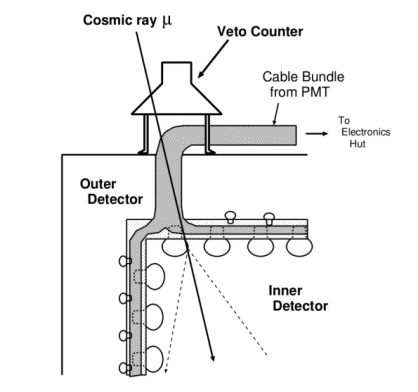
\includegraphics[width=0.5 \textwidth,keepaspectratio=true]{figures/Cable_muon.png}
\caption{Holes in OD PMT coverage, through which cosmic ray muons can pass with minimal OD activity \cite{Gustafson:2016dh}.}
\label{fig:cable_muon}
\end{figure}
\par
In order to remove low energy events, a time-of-flight (TOF) based ``point-fit" vertex fitter is used to select a vertex for the event.  This fitter is a timing based fitter, which searches for a vertex in the detector which minimizes spread in the residual time distribution of PMT hits.  PMT hits are TOF subtracted to this ``point-fit" vertex, and the following cut is applied:
\begin{itemize}
\item The number of ID hits in a sliding 50 ns residual time window must be 50 or more (25 or more for SK-II).
\end{itemize}
Low energy events can evade this cut if they occur in coincidence with a cosmic ray muon.  If the muon arrive just after the low energy event, the energy deposited by the muon allows the event to pass cuts meant to remove low energy events, while the hits in the OD occur to late to be picked up on by OD cuts up to this point.  To remove these ``coincidence muon" events, the following cut is applied:
\begin{itemize}
\item If there are 5,000 or more pe in the ID (2,500 or more for SK-II), there must be fewer than 20 OD hits between +300 ns and +800 ns.
\end{itemize}  
\par
Another type of event which must be removed are so-called ``flasher" events.  These are events where an individual PMT experience an electrical discharge which produces some light, which can be detected by the PMTs around it.  These flasher events generally have longer tails in their timing distributions than true neutrino events.  To search for flashers, the minimum number of ID hits in a 100 ns sliding window which searches in the region from +200 ns to +700 ns is found.  The following cut is then applied
\begin{itemize}
\item (For SK II-IV) The minimum number of ID hits in the 100 ns sliding window must be less than 20.
\item (For SK-I) The minimum number of ID hits in the 100 ns sliding window must be less than 10, unless there are more than 800 ID hits, in which case the minimum number of ID hits in the 100 ns sliding window must be less than 15.
\end{itemize}
The long tail of flasher events makes this fitter perform poorly, so the following cut is also applied to remove flasher events:
\begin{itemize}
\item The point-fit goodness must be great than 0.4
\end{itemize}
\par
Of the about 900 events that pass FC2 each day, only about 80 pass FC3.  The complex reconstruction software ``APFIT", which will be described in detail in \cref{ch:event_reconstruction}, is applied to all events which pass FC3.
\subsection{FC4}
FC4 specifically targets flasher events which have made it through the flasher cuts in FC3.  The algorithm used in FC4 is based on the idea that flasher tubes will result in multiple events with very similar hit patterns.  A database of events is maintained, and each event is compared to events in the database.  To compare events, two variables are used.  First a variable $r$ is computed, which represents the spacial correlation between two events.  The ID wall is segmented into patches about 4 m$^2$ in size.  Comparing two events $A$ and $B$, $    r$ is calculated as:
\begin{equation}
r=\frac{1}{N} \sum \limits_i^N \frac{(Q_i^A-<Q^A>)\times(Q_i^B-<Q^B>)}{\sigma^A \sigma^B}
\end{equation}
where $N$ is the number of patches, $Q_i$ is the summed charge (in pe) in the $i^th$ patch, and $\sigma$ is the RMS of $Q_i$.  The variable $r$ is then increased by 0.15 if the highest charge tube in events A and B is the same.  Next, a variable $d_{ks}$ is calculated, which is the Kolmogorov-Smirnov test applied to the distribution of charge in the different patches.  For a particular event, the 10 largest values of $r$ and smallest values of $d_{ks}$ (large values or $r$ and small values of $d_{ks}$ indicate similar hit patterns) are used to compute a likelihood variable based on the expectation for flasher events.  If the likelihood variable is greater than a cut threshold, then the event is removed, as shown in \cref{fig:flasher_cut}.  FC4 removes a few events each day.   
\begin{figure}
\centering
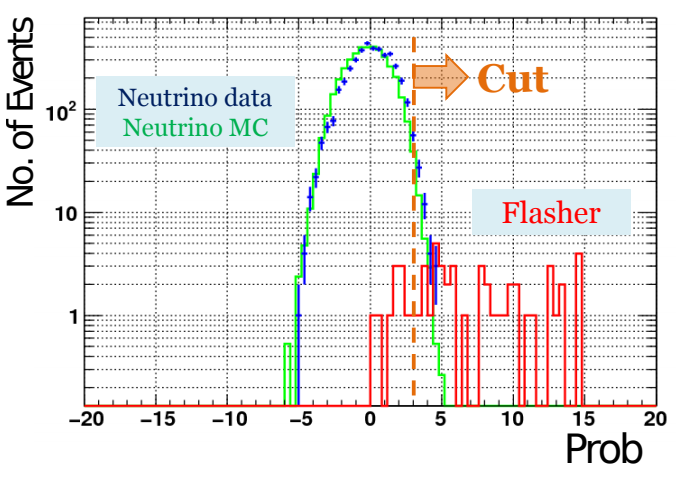
\includegraphics[width=0.5 \textwidth,keepaspectratio=true]{figures/Flasher_cut.png}
\caption{Likelihood variable used for flasher cut in FC5 \cite{Richardson:2015kd}.}
\label{fig:flasher_cut}
\end{figure}
\subsection{FC5}
FC5 focuses on a removing a few particular types of events from the final sample.  First are muons which drop below Cherenkov threshold while traversing the OD.  Known as ``invisible" muons, these can leave minimal activity in the OD, but then decay to an electron in the ID which will trigger the detector.   Therefore, if the number of pe in the ID is less than 1000 (500 for SK-II), which corresponds to the maximum energy of a Michel electron, the following procedure is used to remove these events.  Two clusters of OD hits are defined.  One is the number of clustered OD hits in a 200 ns sliding window with searches from -9000 ns to -200 ns.  This cluster corresponds to hits from before the muon dropped below Cherenkov threshold.  The second is the number of clustered OD hits between -200 ns and 300 ns.  If the locations of the two clusters are less than 500 cm apart, then the following cut is applied:
\begin{itemize}
\item The number of hits in the early cluster must be less than 5, or the number of hits in the two clusters combined must be less than 10.
\end{itemize}
Otherwise, the cut is:
\begin{itemize}
\item The number of hits in the early cluster must be less than 10.
\end{itemize}
\par
Coincidence muons which were not removed during FC3 are targeted by the next cut.  If there are fewer than 300 pe in the ID, the following cut is applied:
\begin{itemize}
\item The number of hits in a 200 ns sliding time window search from +300 ns to +2100 ns must be less than 20.
\end{itemize}
This cut searches a wider late time region than the FC3 coincidence muon cut, but only for very low energy events.
\par
An additional set of cuts to remove cable hole muons which passed FC3 is applied for SK-IV only.  If the stopping muon fitter's goodness is greater than 0.4 and there are more than 1000 pe in the ID and the fitted direction of the muon comes from greater than $37^\circ$ above the horizon, the following cut is applied:
\begin{itemize}
\item The distance between the stopping muon fit entry point and the nearest cable hole must be greater than 2.5 m.
\end{itemize}
\par 
There is also a cut based on the APFIT reconstructed direction, aimed at removing stopping muons:
\begin{itemize}
\item There must be fewer than 4 OD hits within 8 m of the APFIT entry point in a 200 ns sliding window between -500 ns and +300 ns.
\end{itemize}
\par
Finally, there is an additional cut to remove flasher events which made it through FC3 and FC4.  This cut is based on a more complex timing based vertex fitter than was used in FC3.  Similarly to the vertex fitter used in FC3, the goodness of the fit is expected to be low for flasher events with long timing tals.  As in FC3, the minimum number of ID hits in a sliding 100 ns window between +200 ns and +700 ns is found.  If the minimum number of hits in the 100 ns window is six or greater, then the following cut is applied:
\begin{itemize}
\item The goodness of the vertex fit must be better than 0.4.
\end{itemize}
For SK II-IV, a looser cut on the goodness is applied if the minimum number of hits in the 100 ns window is less than 6:
\begin{itemize}
\item The goodness of the vertex fit must be better than 0.3.
\end{itemize}
Like FC4, only a few events each day are removed by FC5, leaving an event rate of 50-80 events per day. 
\subsection{Final Analysis Sample}
The events passing FC5 still contain some background, mostly in the form of low energy radioactive background.   To produce the final analysis sample, three final cuts are applied:
\begin{itemize}
\item The distance from the reconstructed vertex to the ID wall must be greater than 2 m.
\item The reconstructed visible energy must be larger than 30 MeV
\item The maximum number of hits in an OD cluster must be less than 16 (less than 10 for SK-II)
\end{itemize}
After these cuts, about 8 events per day remain, which agrees well with MC expectation.  This final analysis sample if called "Fully-Contained Fiducial Volume" (FCFV), and it is estimated that the efficiency of the FCFV selection for selecting neutrino events in the FV which do not penetrate the OD is about 98\%.  The fraction of FCFV events which are background is estimated to be around 0.3\%-0.4\% in SK II-III, and 0.02\% is SK-IV \cite{Richardson:2015kd}.
\section{Partially Contained Reduction}
The partially contained reduction searches for muons that originated in the ID but were able to penetrate into the OD.  Similarly to the FC reduction, this is done in a sequence of five steps, labeled PC1-PC5.  The PC reduction selects about two events every three days from the $10^6$ events recorded by SK.  Between SK-II and SK-III, the top, bottom, and barrel of the OD were optically separated from one another.  This segmentation allowed for a more efficient PC selection from SK-III onward.  I will describe here the PC selection in SK-III and SK-IV, description of the selection for early periods can be in \cite{Dufour:2009ljt}. 
\section{Upward Going Muon Reduction}
\label{sec:upmu}